%% Template for SDP report, adapted from mlp_cw2_template, 2018. 
% test test from github
%% Based on  LaTeX template for ICML 2017 - example_paper.tex at 
%%  https://2017.icml.cc/Conferences/2017/StyleAuthorInstructions

\documentclass{article}
% \usepackage[T1]{fontenc}
\usepackage{amssymb,amsmath}
\usepackage{txfonts}
\usepackage{microtype}
\usepackage{xspace}
\xspaceaddexceptions{\%}
\usepackage{subcaption}
% Lists with less spacing between items
\usepackage{paralist}
\usepackage{tabularx}
\usepackage[normalem]{ulem}
% For figures
\usepackage{graphicx}
\usepackage{subfig} 

% For citations
\usepackage{natbib}

% For algorithms
\usepackage{algorithm}
\usepackage{algorithmic}

% the hyperref package is used to produce hyperlinks in the
% resulting PDF.  If this breaks your system, please commend out the
% following usepackage line and replace \usepackage{mlp2017} with
% \usepackage[nohyperref]{mlp2017} below.
\usepackage{hyperref}
\usepackage{url}
\urlstyle{same}

% Packages hyperref and algorithmic misbehave sometimes.  We can fix
% this with the following command.
\newcommand{\theHalgorithm}{\arabic{algorithm}}


% Set up MLP coursework style (based on ICML style)
\usepackage{mlp2018}
\mlptitlerunning{SDP Demo \demoNumber  Group (\groupNumber)}
\bibliographystyle{icml2017}


\DeclareMathOperator{\softmax}{softmax}
\DeclareMathOperator{\sigmoid}{sigmoid}
\DeclareMathOperator{\sgn}{sgn}
\DeclareMathOperator{\relu}{relu}
\DeclareMathOperator{\lrelu}{lrelu}
\DeclareMathOperator{\elu}{elu}
\DeclareMathOperator{\selu}{selu}
\DeclareMathOperator{\maxout}{maxout}






% \usepackage{test}

%% You probably do not need to change anything above this comment

%% REPLACE the details in the following commands with your details
% \setGroupNumber{4}
% \setGroupName{Sprout.ed}
% \setProductName{Sprout.ed}
% \setDemoNumber{2}
% \setLogoFileName{figs/sprouted_logo.png}
\usepackage{graphicx}

\title{Sprout.ed - User Guide}
\begin{document} 

\maketitle{}

\begin{figure}[h]
    \centering
    
\includegraphics[width=0.3\linewidth]{figs/sprouted_logo.png}
    \label{fig:logo}
\end{figure}



\section{System Overview} \label{sec:overview}
% Yichao
Sprout.ed is an integrated gardening solution targeting office spaces. 
As more and more people are now working extensive hours in offices and labs, we’d like to bring the delightful elements of nature indoors without adding any burden to the office managers who would have to take care of them in the long run.
Our product Sprout.ed integrates plant sowing, caring and a web-app that offers user monitoring of the plant bed, plants wiki and collaborative activities amount office users. With these features, users can even vote for what plants to grow and regularly take home fresh herbs, flowers from Sprout.ed. And they’d never have to worry about their favourite office plants not being taken care of when their building is occupied or when pandemics happen! \\

The rest of the document is structured as follows to provide a comprehensive guide to Sprout.ed:
\begin{itemize}
    \item \textbf{Section \ref{sec:description}} gives an introduction to the parts of the system
    \item \textbf{Section \ref{sec:setup}} provides a tutorial on setting up the fully-functional system from the aforementioned parts
    \item \textbf{Section \ref{sec:detail}} provides the full detail of how to achieve all tasks Sprout.ed is capable of in its daily operations
    \item \textbf{Section \ref{sec:troubleshooting}} lists the potential system faults that users might encounter and a troubleshooting guide.
\end{itemize}



\section{System Description}\label{sec:description}
%An overview of the system (e.g. parts of the robot, interface layout)
% One member from each sub-team
% Rokas Shreyas Sonia

\begin{figure}[h]
    \centering
    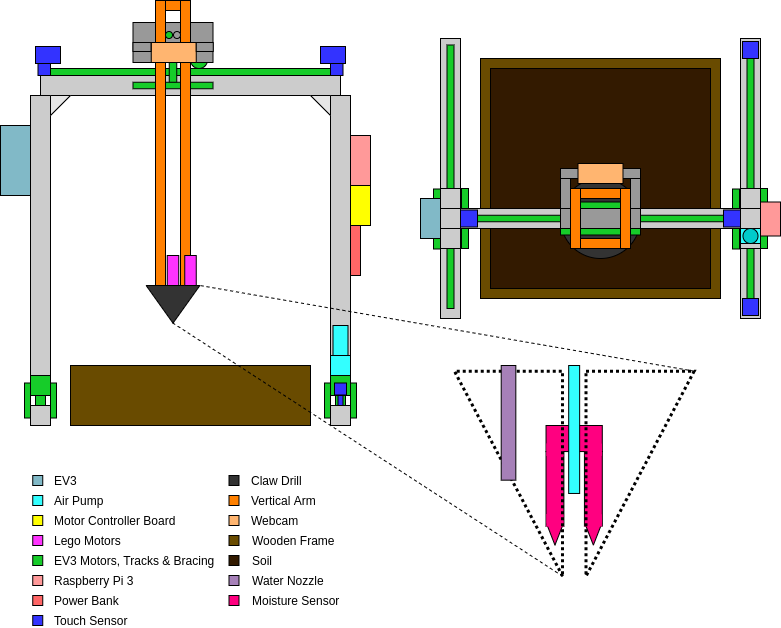
\includegraphics[width=1\linewidth]{figs-userguide/diagram.png}
    \caption{A view of the fully assembled robot from the side (left) and from above (top right), and a zoomed in view of the drill head (bottom right).}
    \label{fig:the-robot}
\end{figure}

\subsection{Hardware}
See Figure \ref{fig:the-robot} for a labelled diagram of how all the components fit together.

\subsection{Electrical}
Sprout.ed's electrical system comprises of a combination of an EV3 and a Raspberry Pi. The EV3 is used for the movement of the gantry and the arm, while the Pi controls the movement of the claw, drop and pickup of seeds, and the 
\subsection{Web Application}
The robot is accompanied by a web application hosted on the Raspberry Pi, which allows for remote monitoring of the plant bed. The app has a User Mode and an Admin Mode. The User Mode can be accessed by any of the office employees, allowing them to see which plants are currently planted, information about them, and a current photograph of the plant. The Admin Mode is designed for office managers, and requires a log in. This Mode additionally allows you to select a new plant type and location to add to the plant bed, check temperature and moisture readings, view actions performed on or by the system, and allows for a manual override watering function.
TODO: Insert screenshot of web app user homepage?

\section{System Setup}\label{sec:setup}
% Unpacking/installation/set up of the hardware and software
% One member from each sub-team
% Anukrat, Terry, Dima
\subsection{Unpacking}

\subsection{Installation}

\subsection{software?}


\section{Operational detail}\label{sec:detail}
% Full details of how to operate the system to achieve all tasks it is capable of (note this might include details relevant to repeated operation such as swapping batteries)
% One member from electrical and webapp
% Sonia, Alan, Rokas

\section{Troubleshooting}\label{sec:troubleshooting}
% A troubleshooting guide (perhaps best presented as a table)
% One member from each sub-team
% Anukrat, Balraj, Serena
Just a list of possible problems ( Rough draft ) \newline
\newline
One side of the gantry is faster than the other \newline
The drill can’t pierce the soil \newline
Camera fails to capture an image \newline
Problem with computer vision \newline
Webapp not displaying \newline
Possible solution - check you are using the right url \newline
No internet connection \newline
Motors not moving \newline
Sensors not working \newline
Raspi web server crashes \newline
Ev3 and raspi no communication \newline
One of the warnings displaying \newline
EV3 disconnected from wifi \newline
Override button might return a timeout error due to disconnection in the pipe \newline
Possible solution: User needs to connect EV3 to the wifi and then ssh into the pi and check if its connected to the wifi. The user should then ensure if all the connections are intact \newline
Air pump might not suck seeds because low battery \newline
Possible solution : Change the batteries \newline




%% Include any references in a bibliography

\bibliography{example-refs}

\end{document} 

